\documentclass[a4paper,12pt]{article}

\usepackage{../latex/mystyle}
\addbibresource{ref.bib}

\begin{document}

\begin{center}
\begin{tabu} to \textwidth {lX[c]r}
    Groupe 1211 & \large{\textbf{Rapport~2}} & 14 octobre 2014 \\
    \hline
\end{tabu}
\end{center}

\section{Introduction}

Notre sujet d'étude étant la production d’ammoniac, en commençant par la synthèse de celui-ci à partir du reformage, il nous a été nécessaire de passer par l’étape de la gestion du plant. Ce rapport présente donc nos calculs et codes MATLAB du bilan de matière, en fonction de la température dans le réacteur et de la quantité d’ammoniac produite, du bilan d’énergie et finalement le calcul du nombre de tubes nécessaires à l’entrée des différents réactifs. 

\section{Flow-sheet rempli}

La figure~\ref{fig:flowsheet2} présente le flow-sheet que nous avons complété à l'aide des sources \cite{epa} et \cite{process-patent}.

\begin{figure}
    \centering
    \tikzstyle{reaction} = [
    rectangle, draw, thick, rounded corners, fill=black!10,
    text width=13em, text centered,
    minimum height=6em
]
\tikzstyle{inout} = [
    rectangle,
    node distance=6em,
    font=\footnotesize
]
\tikzstyle{ioside} = [
    inout,
    node distance=10em
]

\tikzstyle{thinflow} = [
    draw, -latex'
]
\tikzstyle{flow} = [
    thinflow, thick
]

\tikzstyle{flowing} = [
    text centered,
    font=\footnotesize,
    inner sep=.5em,
]

\begin{tikzpicture}[node distance=9em, auto]
    
    % Reaction boxes
    \node [reaction] (primary) {
        Reformage primaire \\[.3em]
        \footnotesize{
            (A) \ce{CH4 + H2O <-> CO + 3H2} \\
            (B) \ce{CO + H2O <-> CO2 + H2} \\
            (équilibre à la sortie)
        }
    };
    \node [reaction, below of=primary] (secondary) {
        Reformage secondaire \\[.3em]
        \footnotesize{
            (C) \ce{2CH4 + O2 -> 2CO + 4H2} \\
            (considérée complète)
        }
    };
    \node [reaction, below of=secondary] (shift) {
        Réacteurs Water-Gas-Shift \\[.3em]
        \footnotesize{
            (D) \ce{CO + H2O -> CO2 + H2} \\
            (considérée complète)
        }
    };
    \node [reaction, below of=shift] (sepa) {
        Séparation de \ce{CO2} et \ce{H2O} \\[.3em]
        \footnotesize{
            (considérée complète)
        }
    };
    \node [reaction, below of=sepa] (synthesis) {
        Synthèse de l'ammoniac et séparation \\
        \footnotesize{
            (E) \ce{N2 + 3H2 -> 2NH3} \\
            (considérée complète)
        }
    };
    \node [reaction, right of=primary, node distance=18em, fill=red!10] (oven)
    {
        Four \\[.3em]
        \footnotesize{
            \ce{CH4 + 2O2 -> CO2 + 2H2O} \\
            (complète)
        }
    };
    
    % Empty in-out boxes
    \node [inout, above of=primary] (in12) {\ce{CH4}, \ce{H2O}};
    \node [ioside, left of=secondary] (in3) {air};
    \node [ioside, right of=sepa, node distance=11em] (out12) {\ce{CO2}, \ce{H2O}};
    \node [ioside, right of=synthesis] (out3) {\ce{Ar}};
    \node [inout, below of=synthesis] (out4) {\ce{NH3}};
    \node [inout, above of=oven] (inoven) {\ce{CH4}, \ce{O2}};
    \node [inout, below of=oven] (outoven) {\ce{CO2}, \ce{H2O}};
    
    % In-out flows (thin arrows)
    \path [thinflow] (in12) -- (primary);
    \path [thinflow] (in3) -- (secondary);
    \path [thinflow] (sepa) -- (out12);
    \path [thinflow] (synthesis) -- (out3);
    \path [flow] (synthesis) -- (out4);
    \path [thinflow] (inoven) -- (oven);
    \path [thinflow] (oven) -- (outoven);

    % Energy flow
    \path [thinflow] (oven) --
    node [flowing, above] {chaleur}
    (primary);

    % Main flows
    \path [flow] (primary) --
    node [flowing, right]{
        \ce{CH4}, \ce{H2O}, \ce{CO}, \ce{CO2}, \ce{H2}
    }
    (secondary); 
    \path [flow] (secondary) --
    node [flowing, right]{
        \ce{H2O}, \ce{CO}, \ce{CO2}, \ce{H2}, \ce{N2}, \ce{Ar}
    }
    (shift);
    \path [flow] (shift) --
    node [flowing, right]{
        \ce{H2O}, \ce{CO2}, \ce{H2}, \ce{N2}, \ce{Ar}
    }
    (sepa);
    \path [flow] (sepa) --
    node [flowing, right]{
        \ce{H2}, \ce{N2}, \ce{Ar}
    }
    (synthesis);

\end{tikzpicture}

    \caption{Flow-sheet simplifiée du procédé de production d'ammoniac.}
    \label{fig:flowsheet2}
\end{figure}
%\begin{figure}
%    \centering
%    \input{flowsheet-matter.tex}
%    \caption{Flow-sheet simplifiée du procédé de production d'ammoniac.}
%    \label{fig:flowsheet-matter}
%\end{figure}

\section{Bilan de matière}

Dans cette section nous allons utiliser ce que nous savons
sur les réactions pour trouver les différents débits de matière du procédé
en fonction du débit sortant de \ce{NH3}
et de la température du réformage primaire.

Il suffit a priori de prendre ce débit
d’ammoniac désiré et remonter pas à pas
dans les différentes équations en se servant des proportions stœchiométriques
(technique dite \emph{bottom-up})
pour déterminer les réactifs de base
et ainsi savoir de combien de moles, ou de kilogrammes, de matière première
nous avons besoin.

Cependant, l'utilisation de cette technique est rendue plus difficile par
l'ajout de réactifs ou l'extraction de produits dans des quantités inconnues
à plusieurs endroits du procédé, ainsi que par les réactions à l'équilibre,
dont l'avancement dépend de la température.

Nous avons donc cherché une solution plus générale et automatique,
qui consiste à résoudre dans un système toutes les équations linéaires homogènes
pour se concentrer ensuite sur la résolution des équations plus compliquées,
avec un nombre plus petit de variables.

\subsection{Inconnues et équations}

Commençons par déterminer nos inconnues et les relations dont nous disposons.

Pour les inconnues, nous choisissons les débits de moles suivants:
\begin{itemize}
    \item $\mbox{in}_\ce{CH4}$, $\mbox{in}_\ce{H2O}$
        et $\mbox{in}\ind{air}$
        les débits d'entrée de \ce{CH4}, \ce{H2O} et air;
    \item $\mbox{out}_\ce{H2O}$, $\mbox{out}_\ce{CO2}$,
        $\mbox{out}_\ce{Ar}$ et $\mbox{out}_\ce{NH3}$
        les débits de sortie de \ce{H2O}, \ce{CO2}, \ce{Ar} et \ce{NH3};
    \item $\alpha$, $\beta$, $\gamma$, $\delta$ et $\epsilon$
        les degrés d'avancement par unité de temps
        des réactions A, B, C, D et E comme notées sur le flow-sheet.
\end{itemize}
Il s'agit bien de débits, que nous exprimerons en $\mole\per\second$,
car le procédé fonctionne en continu.

En ce qui concerne les équations, nous pouvons exprimer:
\begin{itemize}
    \item la non-accumulation de chacune des 9 espèces à travers le procédé:
        ce qui est apporté ou produit doit égaler
        ce qui est enlevé ou ce qui réagit;
    \item le débit de sortie de \ce{NH3}, imposé par l'utilisateur;
    \item les deux relations d'équilibre à la sortie du réacteur de réformage
        primaire.
\end{itemize}

Nous avons $3+4+5 = 12$ inconnues et $9+1+2 = 12$ équations,
donc le système est résolvable.

Les différentes inconnues et équations sont illustrées dans
la figure~\ref{fig:flows-matter}.
Les inconnues (entrées, sorties et réactions) sont représentées par des cercles,
tandis que les 9 relations de conservation de matière
sont représentées par des flèches entre les inconnues.

\begin{figure}
    \centering
    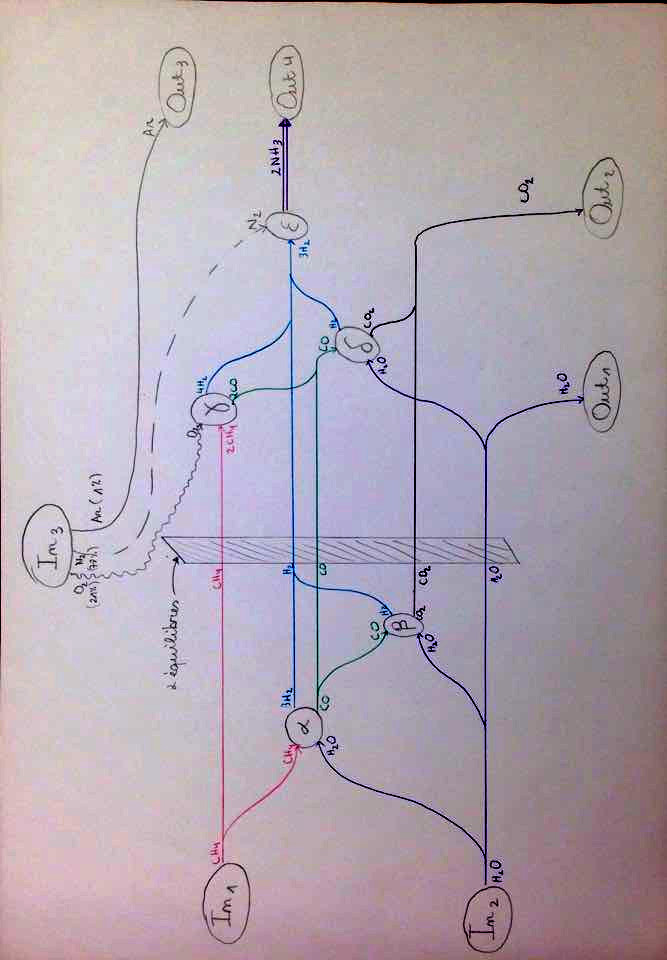
\includegraphics[width=.9\textwidth]{flows_matter}
    \caption{
        Procédé de production du point de vue de la matière.
        On remarque que les relations d'équilibres s'appliquent après que les deux
        réactions du reformage primaire aient eu lieu.
    }
    \label{fig:flows-matter}
\end{figure}

\subsection{Expression des équations}

Maintenant que nous nous sommes assurés que le système est résolvable,
il faut exprimer les différentes équations.

\subsubsection{Non-accumulation des espèces}

Nous allons commencer par les 9 équations de non-accumulation des composés.

Prenons pour commencer l'exemple du \ce{CH4}.
On peut voir sur le flow-sheet (figure~\ref{fig:flows-matter}) que le \ce{CH4}:
\begin{itemize}
    \item entre au début du procédé, à un débit $\mbox{in}_\ce{CH4}$,
    \item est consommé par la réaction A, à un débit $\alpha$,
    \item et le reste est consommé par la réaction C, à un débit $2\gamma$%
        \footnote{Le 2 ici provient du coefficient stœchiométrique du \ce{CH4}}.
\end{itemize}

Dès lors, en appliquant la relation générale de non-accumulation:
\begin{equation*}
    \mbox{entrée} + \mbox{production} = \mbox{sortie} + \mbox{consommation}
\end{equation*}

On obtient la relation liée au \ce{CH4}:
\begin{equation*}
    \mbox{in}_\ce{CH4} \quad + \quad 0 \quad
    = \quad 0 \quad + \quad \alpha + 2\gamma
\end{equation*}

Prenons ensuite l'exemple du \ce{CO2}.
On peut voir sur le flow-sheet que le \ce{CO2}
\begin{itemize}
    \item est produit par la réaction B, à un débit $\beta$,
    \item est produit par la réaction D, à un débit $\delta$.
    \item sort du procédé au niveau de la séparation,
        à un débit $\mbox{out}_\ce{CO2}$.
\end{itemize}

En appliquant la relation générale, on obtient celle liée au \ce{CO2}:
\begin{equation*}
    0 \quad + \quad \beta + \delta \quad
    = \quad \mbox{out}_\ce{CO2} \quad + \quad 0
\end{equation*}

Les autres relations de non-accumulation s'obtiennent de manière similaire,
et sont recueillies dans ce système:
\begin{equation*}
    \left\{
    \begin{array}{rcll}
        \mbox{in}_\ce{CH4} &=& \alpha + 2\gamma
            & \mbox{(\ce{CH4})}\\
        \mbox{in}_\ce{H2O} &=& \mbox{out}_\ce{H2O} + \alpha + \beta + \delta
            & \mbox{(\ce{H2O})}\\
        3\alpha + \beta + 4\gamma + \delta &=& 3\epsilon
            & \mbox{(\ce{H2})}\\
        \alpha + 2\gamma &=& \beta + \delta
            & \mbox{(\ce{CO})}\\
        \beta + \delta &=& \mbox{out}_\ce{CO2}
            & \mbox{(\ce{CO2})}\\
        21\% \times \mbox{in}\ind{air} &=& \gamma
            & \mbox{(\ce{O2})}\\
        78\% \times \mbox{in}\ind{air} &=& \epsilon
            & \mbox{(\ce{N2})}\\
        1\% \times \mbox{in}\ind{air} &=& \mbox{out}_\ce{Ar}
            & \mbox{(\ce{Ar})}\\
        2\epsilon &=& \mbox{out}_\ce{NH3}
            & \mbox{(\ce{NH3})}\\
    \end{array}
    \right.
\end{equation*}

\subsection{Résolution des équations}

La méthode de résolution des équations a été déterminée par le type des équations:
\begin{itemize}
    \item les neuf équations de conservation de masses sont linéaires et homogènes;
    \item l'équation qui impose la sortie de \ce{NH3} est linéaire et non-homogène;
    \item les équations d'équilibre ne sont pas linéaires.
\end{itemize}

Elles sont ici triées dans l'ordre de difficulté croissante.
Nous avons décidé dans notre programme de les résoudre dans cet ordre:
\begin{enumerate}
    \item Les neuf équations linéaires homogènes sont résolues,
        laissant trois degrés de liberté.
        On exprime les solutions sous la forme $av_1 + bv_2 + cv_3$
        où $a$, $b$ et $c$ sont des paramètres de débit inconnus.
        Cette étape est effectuée par la fonction \texttt{param\textunderscore moles}.
    \item Ensuite on impose que la sortie de \ce{NH3} soit égale la valeur entrée.
        Dans notre cas, cela déterminait le paramètre $c$.
        Ceci est une des étapes de la fonction \texttt{solve\textunderscore equi}.
    \item Enfin on résout les équations d'équilibre pour trouver les deux derniers
        paramètres $a$ et $b$. C'est la deuxième partie de la fonction \texttt{solve\textunderscore equi}.
        Notons que les débits à l'équilibre ont dû être préalablement exprimés en fonction
        de $a$, $b$ et $c$, ce qui est le rôle de \texttt{param\textunderscore moles\textunderscore eq}.
\end{enumerate}

Une fois les paramètres $a$, $b$ et $c$ calculés, nous pouvons déduire tous les débits
molaires du procédé, et une fois ceux-là obtenus,
les débits massiques et les chaleurs produites ou absorbées par chacune des réactions.
C'est le rôle de la fonction \texttt{masses\textunderscore and\textunderscore heat},
qui prend simplement en paramètre la température en kelvin et le débit en \kilogram\per\second.

Celle-ci est utilisée directement par l'interface graphique.

\section{Bilan d'énergie}

Nous allons maintenant déterminer la quantité de CH4 qu’il nous faut introduire
dans le four afin de produire l’énergie nécessaire aux réactions
au niveau du reformage primaire pour une quantité de moles demandée.  

Tout d’abord, les réactions au sein de ce réacteur sont globalement endothermiques.
Elles ont donc besoin de recevoir une certaine quantité d’énergie
déterminée par leur enthalpie de réaction respective.
La combustion quant à elle est exothermique et c’est elle qui va fournir cette énergie.
Nous ferons l’hypothèse qu’il n’y aura pas de pertes d’énergie
entre le four et le reformage primaire.

On peut donc exprimer la conservation d'énergie:
$$\alpha*\Delta H_1 + \beta*\Delta H_2 + \xi*\Delta H\ind{four} = 0$$
où $\alpha$, $\beta$ et $\xi$ sont les degrés d'avancement en \mole\per\second,
et $\Delta H_1$, $\Delta H_2$ et $\Delta H_3$ les enthalpies molaires en
\joule\per\mole des trois réactions.
Les degrés d'avancement $\alpha$ et $\beta$ ont été calculées
au préalable pour la quantité d’ammoniac désirée.


\subsection{Calcul des différentes enthalpies à une température $T$}

Pour calculer les différences d'enthalpie des différents composés,
nous utilisons une des formes de l'équation de Shomate \cite{nist}:
$$\Delta H(t) = A\,t + B\,\frac{t^2}{2} + C\,\frac{t^3}{3}
+ D\,\frac{t^4}{4} - E\,\frac{1}{t} + F$$
où $A$, $B$, $C$, $D$, $E$ et $F$ sont des coefficients
%\footnote{Ces coefficients se retrouvent dans l'annexe}
qui dépendent du composé en question et où $t=\frac{T(\kelvin)}{1000}$.

Cette équation donne la différence d'enthalpie entre le composé à la température $T$
et sa forme élémentaire à une température standard $T\ind{ref} = 298.15\,\kelvin$.


\subsubsection{Réactions reformage primaire}

Nous allons considérer ici que les réactifs et les produits sont tous les deux
à une température $T$ (avoisinant ici les $1000\,\kelvin$).


\textbf{Réaction 1 :}  \ce{CH4 + H2O -> CO + 3H2}
\begin{equation*}
    \Delta H_1 (T) = 3*\Delta H_{\ce{H2}} (t)
    + \Delta H_{\ce{CO}} (t)
    - \Delta H_{\ce{CH4}} (t)
    - \Delta H_{\ce{H2O}} (t) 
\end{equation*}

\textbf{Réaction 2 :}  \ce{CO + H2O -> CO2 + H2}
\begin{equation*}
    \Delta H_2 (T) = \Delta H_{\ce{CO2}} (t)
    + \Delta H_{\ce{H2}} (t)
    - \Delta H_{\ce{CO}} (t)
    - \Delta H_{\ce{H2O}} (t) 
\end{equation*}

Chaque $\Delta H$ correspond à l’équation de Shomate
avec les coefficients correspondant au composé en question.


\subsubsection{Dans le four}

Pour la combustion, nous allons considérer que nous apportons les réactifs
à température ambiante, soit $298.15\,\kelvin$,
et que les produits sortent à une température $T\ind{four}=1300\,\kelvin$.

Pour établir le $\Delta H$ de cette réaction,
il suffit une nouvelle fois d’appliquer l’équation de Shomate des produits à température T
et d’y soustraire l’enthalpie de formation à température ambiante de chacun des réactifs,
le tout pondéré par les coefficients stoechiométriques.


\textbf{Réaction Four :}  \ce{CH4 + 2O2 -> CO2 + 2H2O}
\begin{equation*}
    \Delta H\ind{four}(T) =  \Delta H_{\ce{CO2}} (t)
    + 2*\Delta H_{\ce{H2O}} (t)
    - \Delta H\ind{form, \ce{CH4}}
    - 2*\Delta H\ind{form, \ce{O2}}
\end{equation*}


\subsubsection{Cas pour une température particulière}


Appliquons formules explicitées ci-dessus pour les températures $T=1000\,\kelvin$
dans le réacteur et $T\ind{four} = 1300\,\kelvin$ dans le four,
pour se donner une idée des valeurs auxquelles s'attendre:

$$\Delta H_1 (1000\,\kelvin) = 225.72\,\kilo\joule\per\mole$$

$$\Delta H_2 (1000\,\kelvin) = -34.779\,\kilo\joule\per\mole$$

$$\Delta H\ind{four}  (1300\,\kelvin) = -674.28\,\kilo\joule\per\mole$$


A présent, il nous reste à trouver le degré d'avancement $\xi$
qui nous donnera les débits des réactifs et des produits de la combustion :
$$\xi = \frac{\alpha * \Delta (H_1) + \beta * \Delta (H_2)}{\Delta (H_3)}$$
où $\xi$ donnera le débit de \ce{CH4} et de \ce{CO2},
2$\xi$ donnera le débit de \ce{O2} et de \ce{H2O}.


Enfin, pour obtenir le débit de réactifs à introduire dans le four,
il suffira de multiplier chacun des flux par la masse molaire des composés respectifs :
\begin{equation*}
    M_{\ce{CH4}}=16.0425\,\gram\per\mole \mbox{ et } M_{\ce{O2}}=31.9988\,\gram\per\mole
\end{equation*}

\section{Analyse paramétrique}

Tout ce que nous avons calculé et modélisé nous permet maintenant de faire une analyse paramétrique de notre système, pour voir son évolution en fonction de la température et de la quantité de \ce{NH3} désirée.

Nous avons choisi de faire varier la température entre $900\,\kelvin$ et $1100\,\kelvin$, ce qui constitue une gamme des températures les plus probables, et tout ceci pour une même masse d'ammoniac synthétisé.
Nous n'avons pas jugé utile de faire un graphique pour différentes masses de \ce{NH3} car les entrées et sorties sont proportionnelles à celles-ci, et un tel graphique n'aurait donc pas été très intéressant.

Nous présentons nos conclusions sur la figure~\ref{fig:graphe}.

\begin{figure}
    \begin{center}
        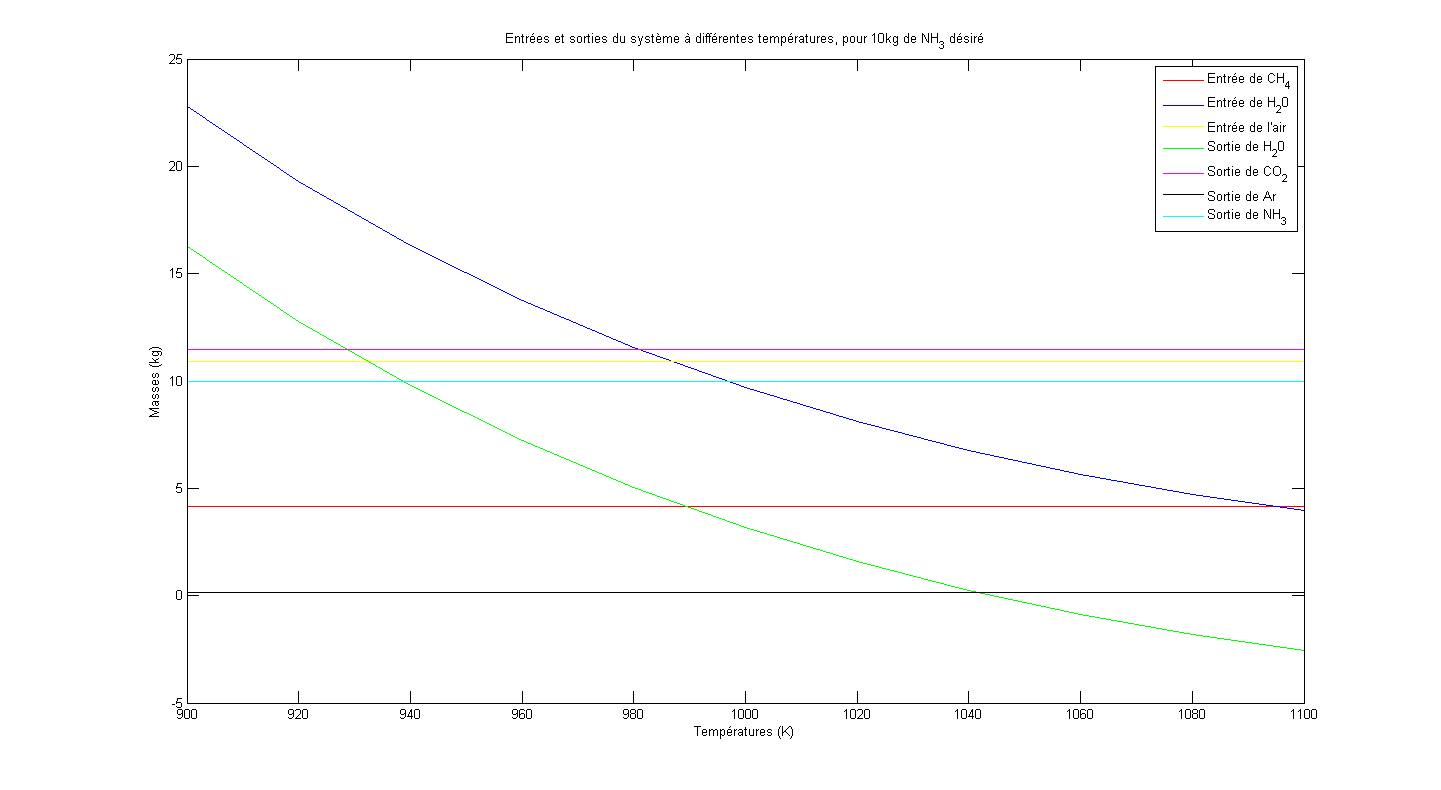
\includegraphics[width=\textwidth]{graphe1}
        \caption{On peut observer sur ce graphique que seules les entrées et sorties de
            \ce{H2O} varient.
            En effet, toutes les autres entrées et sorties sont directement
            liées à la quantité de \ce{NH3} désirée.
            Celles-ci sont donc constantes sur notre graphique.
            On peut également observer que la sortie de \ce{H2O} devient négative
            à la température de $1045\,\kelvin$.
            Le système a en fait besoin, à partir de cette température,
            de plus d'eau dans le reformage secondaire.
        }
        \label{fig:graphe}
    \end{center}
\end{figure}

\section{Nombre de tubes du réacteur}

Dans cette partie, nous allons estimer le nombre de tubes opérés
en parallèle pour apporter le méthane à l'entrée du réacteur de reformage primaire.

L’énoncé nous indique que pour une capacité de $1500\,\ton\per\jour$ d’ammoniac,
la vitesse superficielle typique à l’entrée du réacteur de reformage
à vapeur de méthane est typiquement de $2\,\meter\per\second$.
Nous savons que les tubes sont circulaires et leur diamètre est $10\,\centi\meter$.

Nous prenons également pour les besoins du raisonnement
une pression de $31\,\bbar$ et une température de $1000\,\kelvin$
à l'endroit concerné.

Pour commencer, nous pouvons aisément déduire le débit volumique pour un tube,
comme le produit de la vitesse $c$, et de la section du tube $A$.
Nous obtenons:
\begin{equation*}
    \dot{V}\ind{tube} = c*A = 2\,\meter\per\second \times \pi(0.05\,\meter)^2
    = 0.0157\,\meter\cubed\per\second
\end{equation*}

Ensuite, calculons le débit molaire de \ce{NH3} à la sortie
à partir du débit massique $\dot{m} = 1500\,\ton\per\jour = 17.36\,\kilogram\per\second$.
En divisant ce dernier par la masse molaire de \ce{NH3} ($0.017\kilogram\per\mole$),
on obtient un débit de:
\begin{equation*}
    \dot{n}\ind{sortie} = \frac{\dot{m}}{M_{\ce{NH3}}}
    = \frac{17.36\,\kilogram\per\second}{0.017\,\kilogram\per\mole}
    = 1021.18\,\mole\per\second
\end{equation*}

En utilisant la fonction \texttt{moles} de notre outil de gestion,
nous déterminons les débits molaires à l'entrée du réacteur:
\begin{equation*}
    \dot{n}\ind{entrée} = 451.7\,\mole\per\second
\end{equation*}

Maintenant, calculons le débit volumique total, $\dot{V}$.
Appliquons pour cela la loi des gaz parfaits:
\begin{equation*}
    \dot{V} = \frac{\dot{n}\ind{entrée}RT}{p} = 1.211\,\meter\cubed\per\second
\end{equation*}

Pour finir, nous pouvons déterminer
le nombre de tubes nécessaire avec la relation suivante:
\begin{equation*}
    \frac{\dot{V}}{\dot{V}\ind{tube}}
    = \frac{1.211\,\meter\cubed\per\second}{0.0157\,\meter\cubed\per\second} = 77.16
\end{equation*}
Nous concluons donc qu'environ 80 tubes seront nécessaires pour apporter le méthane
dans le réacteur de reformage primaire.

\section{Outil de gestion}

L'outil de gestion est fourni sous la forme d'un archive ZIP à côté de ce PDF.
La fonction à utiliser est \texttt{masses\textunderscore and\textunderscore heat},
qui prend simplement en paramètre la température en kelvin et le débit
de \ce{NH3} en \kilogram\per\second.

Nous avons développé une ébauche d'interface pour cette fonction,
mais nous préférons reporter sa publication à un moment du projet où nous aurons
une meilleure idée des besoins du projet.

\printbibliography[heading=bibintoc]

\end{document}
